\documentclass[12pt]{article}
\usepackage{setspace, graphicx, fullpage, amssymb, amsmath, epsfig, natbib, array, multirow, hyperref}
\usepackage{amsfonts, bm} 
\usepackage{dcolumn}
\usepackage{subfigure, float} 
\usepackage[margin=.8in]{geometry} 
\usepackage{verbatim}
\usepackage{url}
\usepackage{enumerate}
\usepackage{morefloats}
\newcolumntype{d}[1]{D{.}{.}{#1}} 

\begin{document}
	
\begin{center}
	\Large 15 March 2017
\end{center}

\section{Overview}

At our previous meeting we decided to do the following:

\begin{itemize}
	\item Compare same state Senators who are up for reelection against those who aren't, taking Levitt (1996), Table 4 as inspiration
	
	\item Reconduct analyses with an interaction effect between member vote share and presidential vote share
	
	\item Conduct analyses with noncall response rate (\verb|pfrate100|) as the DV
	
	\item Produce figures which plot our main independent variable (\verb|ideological_extremism|) against party call response rate (\verb|pirate100|) and noncall response rate (\verb|pfrate100|)
\end{itemize}

\noindent
These are included below. For analysis of reelection, William and I settled on a generalized version of difference in differences estimation, further detailed in its subsection. Additionally, I would note that the interaction term for vote share and presidential vote share in some instances receives entirely unrealistic coefficients, and in others which it is included other variables take them.

\section{Tables and Figures}

\subsection{Generalized Difference in Differences Tests}

Our generalized form of the diff in diff uses cases in which there are 2 Senators from a state in a given Congress, one of whom is up for reelection at the end of the Congress and one of whom is not. The effect is calculated by 

With this test, we estimate the effect as well as a placebo derived from a randomly assigned treatment condition. Analysis is provided separately with responsiveness rate to party calls (tables 1 through 3) and responsiveness rate to noncalls (tables 4 through 6) as dependent variables. Within these, we report the estimate for the ATT and the lower and upper bounds of the 95\% confidence interval. The confidence interval is calculated through a bootstrap at the state level. The first table in each set provides a naive calculation of the confidence interval while the second uses weights the effect by seat pair type. The third table provides the estimated effect for each seat pair type.

\pagebreak

% latex table generated in R 3.3.2 by xtable 1.8-2 package
% Mon Mar 13 11:39:19 2017
\begin{table}[H]
	\centering
	\caption{Difference in Differences, Party Influenced Rate, Reelection Treatment vs. Random Assignment}
	\begin{tabular}{llrrr}
		\hline
		Test & DV & Estimate & Lower Bound & Upper Bound \\ 
		\hline
		Effect & pirate100 & -1.5685604 & -2.0957029 & -0.97344617 \\ 
		Placebo & pirate100 & -0.6902020 & -1.2397304 & 1.23271255 \\ 
		\hline
	\end{tabular}
\end{table}

% latex table generated in R 3.3.2 by xtable 1.8-2 package
% Mon Mar 13 00:30:40 2017
\begin{table}[H]
	\centering
	\caption{Weighted Difference in Differences, Party Influenced Rate, Reelection Treatment vs. Random Assignment}
	\begin{tabular}{llrrr}
		\hline
		Test & DV & Estimate & Lower Bound & Upper Bound \\  
		\hline
		Adjusted Effect & pirate100 & -1.5685604 & -2.1541096 & -0.97751751 \\ 
		Adjusted Placebo & pirate100 & -0.6902020 & -6.1688446 & 6.06350669 \\ 
		\hline
	\end{tabular}
\end{table}

% latex table generated in R 3.3.2 by xtable 1.8-2 package
% Mon Mar 13 19:15:44 2017
\begin{table}[H]
	\centering
	\caption{Disaggregated Difference in Differences, Party Influenced Rate, Reelection Treatment vs. Random Assignment}
	\begin{tabular}{llrrr}
		\hline
		Test & DV & Estimate & Lower Bound & Upper Bound \\ 
		\hline
		2 Maj Dems Effect & pfrate100 & 0.0708958 & -1.1103696 & 1.3021792 \\ 
		2 Maj Dems Placebo & pfrate100 & -0.2036783 & -1.3153739 & 2.5118232 \\ 
		\hline
		2 Min Dems Effect & pfrate100 & -1.8733904 & -3.3561696 & -0.3365146 \\ 
		2 Min Dems Placebo & pfrate100 & -0.9602191 & -4.4928217 & 0.0446105 \\ 
		\hline
		2 Maj Reps Effect & pfrate100 & -1.1307379 & -2.7893727 & 0.4274621 \\ 
		2 Maj Reps Placebo & pfrate100 & -0.2868056 & -2.4327395 & 0.8163004 \\
		\hline 
		2 Min Reps Effect & pfrate100 & 0.3990873 & -1.9098626 & 2.7513303 \\ 
		2 Min Reps Placebo & pfrate100 & 0.0147628 & -0.7190561 & 4.9846197 \\ 
		\hline
		Split, Maj Dem Effect & pfrate100 & -2.4804711 & -5.2946938 & 0.1946835 \\ 
		Split, Maj Dem Placebo & pfrate100 & -0.7279546 & -6.5153100 & 0.7413151 \\
		\hline 
		Split, Maj Rep Effect & pfrate100 & -4.3246972 & -7.9137123 & -1.0528934 \\ 
		Split, Maj Rep Placebo & pfrate100 & 0.3390961 & -4.6591781 & 3.0814310 \\
		\hline
	\end{tabular}
\end{table}

\pagebreak

% latex table generated in R 3.3.2 by xtable 1.8-2 package
% Mon Mar 13 11:12:56 2017
\begin{table}[H]
	\centering
	\caption{Difference in Differences, Party Free Rate, Reelection Treatment vs. Random Assignment}
	\begin{tabular}{llrrr}
		\hline
		Test & DV & Estimate & Lower Bound & Upper Bound \\ 
		\hline
		Effect & pfrate100 & -0.2969119 & -0.7350467 & 0.13767116 \\ 
		Placebo & pfrate100 & -0.3120122 & -1.0565962 & 1.06650160 \\  
		\hline
	\end{tabular}
\end{table}

% latex table generated in R 3.3.2 by xtable 1.8-2 package
% Mon Mar 13 11:12:56 2017
\begin{table}[H]
	\centering
	\caption{Weighted Difference in Differences, Party Free Rate, Reelection Treatment vs. Random Assignment}
	\begin{tabular}{llrrr}
		\hline
		Test & DV & Estimate & Lower Bound & Upper Bound \\ 
		\hline
		Adjusted Effect & pfrate100 & -0.2969119 & -0.7111920 & 0.14368690 \\ 
		Adjusted Placebo & pfrate100 & -0.3120122 & -6.5885299 & 6.18565591 \\  
		\hline
	\end{tabular}
\end{table}

% latex table generated in R 3.3.2 by xtable 1.8-2 package
% Mon Mar 13 19:15:44 2017
\begin{table}[H]
	\centering
	\caption{Disaggregated Difference in Differences, Party Free Rate, Reelection Treatment vs. Random Assignment}
	\begin{tabular}{llrrr}
		\hline
		Test & DV & Estimate & Lower\_Bound & Upper\_Bound \\ 
		\hline
		2 Maj Dems Effect & pfrate100 & 0.1900901 & -0.9051052 & 1.2085652 \\ 
		2 Maj Dems Placebo & pfrate100 & -0.9693719 & -2.1048645 & 1.1132629 \\ 
		\hline
		2 Min Dems Effect & pfrate100 & -0.0480525 & -1.4851263 & 1.2185462 \\ 
		2 Min Dems Placebo & pfrate100 & -0.4318845 & -2.0335940 & 2.0935476 \\ 
		\hline
		2 Maj Reps Effect & pfrate100 & 1.0805092 & -0.3291277 & 2.4347626 \\ 
		2 Maj Reps Placebo & pfrate100 & 0.4701269 & -1.5580550 & 2.6796322 \\ 
		\hline
		2 Min Reps Effect & pfrate100 & -0.3783909 & -2.2545156 & 1.5678486 \\ 
		2 Min Reps Placebo & pfrate100 & 0.6484191 & -2.8825838 & 1.8106381 \\ 
		\hline
		Split, Maj Dem Effect & pfrate100 & -1.3097195 & -3.3250855 & 0.6320594 \\ 
		Split, Maj Dem Placebo & pfrate100 & 0.5617371 & -3.3700814 & 2.9765242 \\ 
		\hline
		Split, Maj Rep Effect & pfrate100 & -0.6552082 & -2.9814058 & 1.6811481 \\ 
		Split, Maj Rep Placebo & pfrate100 & 0.3091112 & -4.2642729 & 1.4093758 \\ 
		\hline
	\end{tabular}
\end{table}

\pagebreak

\subsection{Models With Vote Share Interaction}

\begin{table}[H]
	\begin{center}
		\caption{Senate Inter-Party Regression With Vote Share Interaction}
		\begin{tabular}{l c c c c }
			\hline
			& Democrats & Republicans & Majority & Minority \\
			\hline
			ideological\_extremism        & $3.141^{***}$ & $7.798^{***}$ & $4.724^{***}$  & $7.942^{***}$  \\
			& $(0.409)$     & $(0.357)$     & $(0.314)$      & $(0.398)$      \\
			pfrate100                     & $0.758^{***}$ & $0.738^{***}$ & $0.697^{***}$  & $0.685^{***}$  \\
			& $(0.030)$     & $(0.031)$     & $(0.025)$      & $(0.036)$      \\
			pres\_vote\_share $ \times $ vote\_share & $8.236$       & $36.837$      & $33.931^{*}$   & $103.889^{**}$ \\
			& $(19.356)$    & $(31.549)$    & $(16.361)$     & $(32.684)$     \\
			pres\_vote\_share             & $18.121$      & $-35.589$     & $-3.266$       & $-63.056^{**}$ \\
			& $(12.592)$    & $(19.274)$    & $(10.542)$     & $(20.265)$     \\
			vote\_share                   & $-9.240$      & $-6.762$      & $-18.502^{*}$  & $-49.738^{**}$ \\
			& $(9.607)$     & $(18.774)$    & $(8.605)$      & $(18.277)$     \\
			female                        & $1.730^{*}$   & $0.596$       & $0.613$        & $4.474^{***}$  \\
			& $(0.736)$     & $(1.139)$     & $(0.757)$      & $(1.109)$      \\
			afam                          & $-1.149$      & $-10.540^{*}$ & $1.616$        & $-5.209$       \\
			& $(2.790)$     & $(4.283)$     & $(4.177)$      & $(3.203)$      \\
			latino                        & $1.838$       & $7.088^{*}$   & $4.805^{*}$    & $5.847$        \\
			& $(2.199)$     & $(2.783)$     & $(1.875)$      & $(3.489)$      \\
			up\_for\_reelection           & $-0.629$      & $-1.410^{**}$ & $-0.919^{*}$   & $-1.188^{*}$   \\
			& $(0.426)$     & $(0.538)$     & $(0.411)$      & $(0.599)$      \\
			seniority                     & $0.040$       & $-0.016$      & $0.078$        & $0.130$        \\
			& $(0.052)$     & $(0.072)$     & $(0.060)$      & $(0.069)$      \\
			freshman                      & $0.755$       & $0.372$       & $0.574$        & $1.006$        \\
			& $(0.709)$     & $(0.842)$     & $(0.630)$      & $(1.026)$      \\
			retiree                       & $1.602$       & $2.272^{*}$   & $1.851^{*}$    & $2.463^{*}$    \\
			& $(0.897)$     & $(0.997)$     & $(0.849)$      & $(1.105)$      \\
			best\_committee               & $0.235$       & $0.007$       & $0.026$        & $0.331$        \\
			& $(0.124)$     & $(0.154)$     & $(0.118)$      & $(0.174)$      \\
			leader                        & $2.212^{**}$  & $0.869$       & $1.347^{*}$    & $2.023^{*}$    \\
			& $(0.713)$     & $(0.776)$     & $(0.661)$      & $(0.894)$      \\
			power\_committee              & $-0.855$      & $-0.352$      & $-0.094$       & $-1.402$       \\
			& $(0.772)$     & $(0.925)$     & $(0.718)$      & $(1.058)$      \\
			chair                         & $0.864$       & $3.612^{***}$ & $0.002$        &                \\
			& $(0.544)$     & $(0.700)$     & $(0.516)$      &                \\
			south                         & $-1.685^{**}$ & $0.939$       & $0.170$        & $1.362^{*}$    \\
			& $(0.558)$     & $(0.581)$     & $(0.430)$      & $(0.625)$      \\
			(Intercept)                   & $12.094$      & $31.444^{**}$ & $27.678^{***}$ & $47.493^{***}$ \\
			& $(6.866)$     & $(11.882)$    & $(6.060)$      & $(12.213)$     \\
			\hline
			R$^2$                         & 0.689         & 0.642         & 0.685          & 0.619          \\
			Adj. R$^2$                    & 0.684         & 0.635         & 0.680          & 0.612          \\
			Num. obs.                     & 1042          & 951           & 1052           & 843            \\
			RMSE                          & 6.121         & 7.253         & 5.856          & 7.707          \\
			\hline
			\multicolumn{5}{l}{\scriptsize{$^{***}p<0.001$, $^{**}p<0.01$, $^*p<0.05$}}
		\end{tabular}
	\end{center}
\end{table}

\begin{table}[H]
	\begin{center}
		\caption{Senate Intra-Party Regression With Vote Share Interaction}
		\begin{tabular}{l c c c c }
			\hline
			& \multicolumn{2}{c}{Democrats} & \multicolumn{2}{c}{Republicans} \\
			\cline{2-5}
			& Southern & Others & Gingrich Senators & Others \\
			\hline
			ideological\_extremism        & $4.516^{***}$ & $2.635^{***}$ & $3.056^{***}$  & $6.536^{***}$ \\
			& $(1.156)$     & $(0.409)$     & $(0.648)$      & $(0.400)$     \\
			pfrate100                     & $0.850^{***}$ & $0.636^{***}$ & $0.255^{***}$  & $0.823^{***}$ \\
			& $(0.065)$     & $(0.035)$     & $(0.053)$      & $(0.034)$     \\
			pres\_vote\_share $ \times $ vote\_share & $4.879$       & $-19.811$     & $-28.408$      & $61.766$      \\
			& $(35.409)$    & $(26.647)$    & $(39.908)$     & $(35.099)$    \\
			pres\_vote\_share             & $23.336$      & $35.113^{*}$  & $17.874$       & $-42.450^{*}$ \\
			& $(25.009)$    & $(16.522)$    & $(24.739)$     & $(21.393)$    \\
			vote\_share                   & $-5.032$      & $6.756$       & $18.872$       & $-26.916$     \\
			& $(16.781)$    & $(13.862)$    & $(23.437)$     & $(20.963)$    \\
			female                        & $0.231$       & $2.421^{**}$  &                & $2.165$       \\
			& $(1.995)$     & $(0.739)$     &                & $(1.127)$     \\
			up\_for\_reelection           & $-1.548$      & $-0.345$      & $-0.466$       & $-1.725^{**}$ \\
			& $(1.075)$     & $(0.432)$     & $(0.699)$      & $(0.586)$     \\
			seniority                     & $-0.294^{*}$  & $0.138^{*}$   & $-0.277$       & $0.152^{*}$   \\
			& $(0.141)$     & $(0.055)$     & $(0.180)$      & $(0.076)$     \\
			freshman                      & $2.026$       & $0.730$       & $-0.219$       & $0.173$       \\
			& $(1.774)$     & $(0.727)$     & $(0.969)$      & $(0.967)$     \\
			retiree                       & $1.650$       & $1.926^{*}$   & $2.905$        & $2.394^{*}$   \\
			& $(2.260)$     & $(0.925)$     & $(1.617)$      & $(1.047)$     \\
			best\_committee               & $0.570$       & $0.131$       & $0.089$        & $0.043$       \\
			& $(0.310)$     & $(0.129)$     & $(0.182)$      & $(0.177)$     \\
			leader                        & $5.730^{*}$   & $1.764^{*}$   & $1.759$        & $0.835$       \\
			& $(2.319)$     & $(0.695)$     & $(1.144)$      & $(0.839)$     \\
			power\_committee              & $0.762$       & $-1.333$      & $1.064$        & $-1.297$      \\
			& $(2.131)$     & $(0.780)$     & $(1.121)$      & $(1.057)$     \\
			chair                         & $3.101^{*}$   & $0.572$       & $1.291$        & $3.649^{***}$ \\
			& $(1.404)$     & $(0.556)$     & $(1.114)$      & $(0.738)$     \\
			afam                          &               & $-1.035$      &                & $-7.389$      \\
			&               & $(2.494)$     &                & $(4.197)$     \\
			latino                        &               & $2.767$       & $3.077$        & $3.143$       \\
			&               & $(1.969)$     & $(2.535)$      & $(3.611)$     \\
			south                         &               &               & $-0.097$       & $1.114$       \\
			&               &               & $(0.727)$      & $(0.663)$     \\
			(Intercept)                   & $-4.701$      & $14.141$      & $56.912^{***}$ & $30.957^{*}$  \\
			& $(13.273)$    & $(9.099)$     & $(16.065)$     & $(13.116)$    \\
			\hline
			R$^2$                         & 0.728         & 0.572         & 0.238          & 0.679         \\
			Adj. R$^2$                    & 0.712         & 0.563         & 0.172          & 0.672         \\
			Num. obs.                     & 246           & 796           & 188            & 763           \\
			RMSE                          & 7.350         & 5.447         & 4.073          & 7.080         \\
			\hline
			\multicolumn{5}{l}{\scriptsize{$^{***}p<0.001$, $^{**}p<0.01$, $^*p<0.05$}}
		\end{tabular}
	\end{center}
\end{table}

\begin{table}[H]
	\begin{center}
		\caption{Senate Inter-Party Fixed Effects Models With Vote Share Interaction}
		\begin{tabular}{l c c c c }
			\hline
			& Democrats & Republicans & Majority & Minority \\
			\hline
			ideological\_extremism        & $2.87^{***}$ & $3.99^{***}$  & $1.77^{**}$   & $3.86^{***}$ \\
			& $(0.68)$     & $(0.74)$      & $(0.63)$      & $(0.96)$     \\
			pfrate100                     & $0.37^{***}$ & $0.25^{***}$  & $0.37^{***}$  & $0.17^{*}$   \\
			& $(0.05)$     & $(0.05)$      & $(0.05)$      & $(0.07)$     \\
			vote\_share $ \times $ pres\_vote\_share & $22.96$      & $54.35$       & $28.62$       & $57.86$      \\
			& $(23.59)$    & $(30.34)$     & $(30.61)$     & $(30.56)$    \\
			vote\_share                   & $-8.73$      & $-37.15$      & $-12.46$      & $-34.12$     \\
			& $(10.95)$    & $(19.24)$     & $(16.42)$     & $(18.33)$    \\
			pres\_vote\_share             & $11.50$      & $-24.70$      & $10.77$       & $-21.74$     \\
			& $(15.74)$    & $(19.31)$     & $(19.69)$     & $(20.62)$    \\
			freshman                      & $0.66$       & $0.99^{*}$    & $0.68$        & $0.83$       \\
			& $(0.48)$     & $(0.47)$      & $(0.46)$      & $(0.76)$     \\
			retiree                       & $0.20$       & $0.84$        & $0.40$        & $0.60$       \\
			& $(0.83)$     & $(0.82)$      & $(0.99)$      & $(0.90)$     \\
			best\_committee               & $0.13$       & $0.08$        & $0.27$        & $0.32$       \\
			& $(0.12)$     & $(0.16)$      & $(0.15)$      & $(0.18)$     \\
			up\_for\_reelection           & $-0.54^{*}$  & $-1.51^{***}$ & $-0.99^{***}$ & $-1.05^{**}$ \\
			& $(0.27)$     & $(0.35)$      & $(0.28)$      & $(0.37)$     \\
			power\_committee              & $-0.46$      & $-0.20$       & $-1.21$       & $-0.41$      \\
			& $(0.70)$     & $(0.98)$      & $(0.90)$      & $(1.01)$     \\
			leader                        & $0.88$       & $1.43^{*}$    & $1.38$        & $1.37$       \\
			& $(0.49)$     & $(0.61)$      & $(0.77)$      & $(0.78)$     \\
			chair                         & $0.41$       & $0.61$        & $-0.54$       &              \\
			& $(0.65)$     & $(0.71)$      & $(0.55)$      &              \\
			\hline
			Num. obs.                     & 1042         & 951           & 1052          & 843          \\
			R$^2$            & 0.89         & 0.91          & 0.92          & 0.94         \\
			Adj. R$^2$       & 0.87         & 0.88          & 0.89          & 0.91         \\
			\hline
			\multicolumn{5}{l}{\scriptsize{$^{***}p<0.001$, $^{**}p<0.01$, $^*p<0.05$}}
		\end{tabular}
	\end{center}
\end{table}

\begin{table}[H]
	\begin{center}
		\caption{Senate Intra-Party Fixed Effects Models With Vote Share Interaction}
		\begin{tabular}{l c c c c }
			\hline
			& \multicolumn{2}{c}{Democrats} & \multicolumn{2}{c}{Republicans} \\
			\cline{2-5}
			& Southern & Others & Gingrich Senators & Others \\
			\hline
			ideological\_extremism        & $10.72^{***}$ & $2.04^{***}$ & $2.11$    & $4.01^{***}$  \\
			& $(2.58)$      & $(0.56)$     & $(1.52)$  & $(0.86)$      \\
			pfrate100                     & $0.05$        & $0.37^{***}$ & $0.12$    & $0.27^{***}$  \\
			& $(0.15)$      & $(0.06)$     & $(0.11)$  & $(0.06)$      \\
			vote\_share $ \times $ pres\_vote\_share & $25.89$       & $-14.11$     & $-40.08$  & $71.18^{*}$   \\
			& $(31.72)$     & $(26.42)$    & $(24.94)$ & $(36.07)$     \\
			vote\_share                   & $-10.78$      & $12.44$      & $22.12$   & $-48.76^{*}$  \\
			& $(13.70)$     & $(13.97)$    & $(14.85)$ & $(23.22)$     \\
			pres\_vote\_share             & $2.67$        & $22.16$      & $24.92$   & $-32.27$      \\
			& $(25.72)$     & $(18.65)$    & $(19.32)$ & $(23.02)$     \\
			freshman                      & $0.57$        & $1.09^{*}$   & $-0.38$   & $1.55^{*}$    \\
			& $(0.91)$      & $(0.51)$     & $(0.85)$  & $(0.60)$      \\
			retiree                       & $-2.93$       & $0.89$       & $1.47$    & $0.73$        \\
			& $(2.11)$      & $(0.64)$     & $(1.06)$  & $(0.92)$      \\
			best\_committee               & $0.46$        & $0.04$       & $0.32$    & $0.02$        \\
			& $(0.32)$      & $(0.12)$     & $(0.30)$  & $(0.18)$      \\
			up\_for\_reelection           & $-0.41$       & $-0.46$      & $-0.62$   & $-1.73^{***}$ \\
			& $(0.72)$      & $(0.28)$     & $(0.55)$  & $(0.41)$      \\
			power\_committee              & $-2.01$       & $-0.10$      & $-0.88$   & $0.17$        \\
			& $(2.23)$      & $(0.66)$     & $(1.20)$  & $(1.14)$      \\
			leader                        & $2.65$        & $0.76$       & $0.97$    & $1.47^{*}$    \\
			& $(2.16)$      & $(0.49)$     & $(0.89)$  & $(0.72)$      \\
			chair                         & $1.84$        & $0.30$       & $-1.00$   & $0.73$        \\
			& $(1.66)$      & $(0.60)$     & $(0.95)$  & $(0.82)$      \\
			\hline
			Num. obs.                     & 246           & 796          & 188       & 763           \\
			R$^2$           & 0.91          & 0.87         & 0.66      & 0.91          \\
			Adj. R$^2$      & 0.87          & 0.84         & 0.50      & 0.88          \\
			\hline
			\multicolumn{5}{l}{\scriptsize{$^{***}p<0.001$, $^{**}p<0.01$, $^*p<0.05$}}
		\end{tabular}
	\end{center}
\end{table}

\begin{figure}[H]
	\centering
	\caption{House Ideological Extremism Coefficient Plot, Majority}
	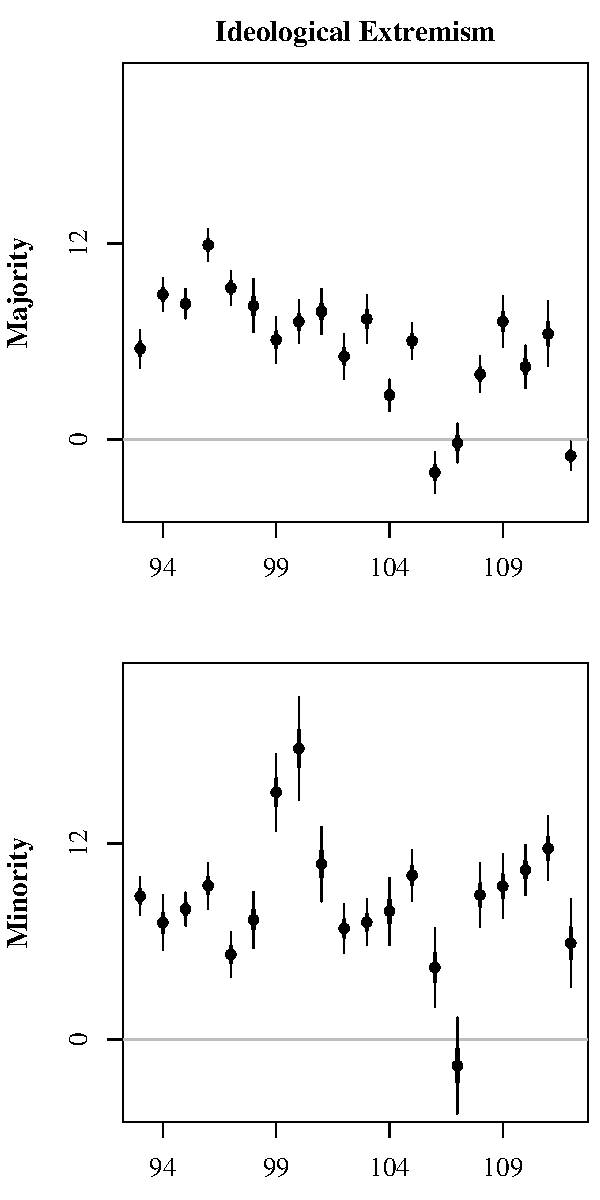
\includegraphics[width = 10cm]{C:/Users/Ethan/Documents/GitHub/partycalls/plots/who-heeds-figure2-replication_interaction.pdf}
\end{figure}

\begin{figure}[H]
	\centering
	\caption{House Ideological Extremism Coefficient Plot, Party}
	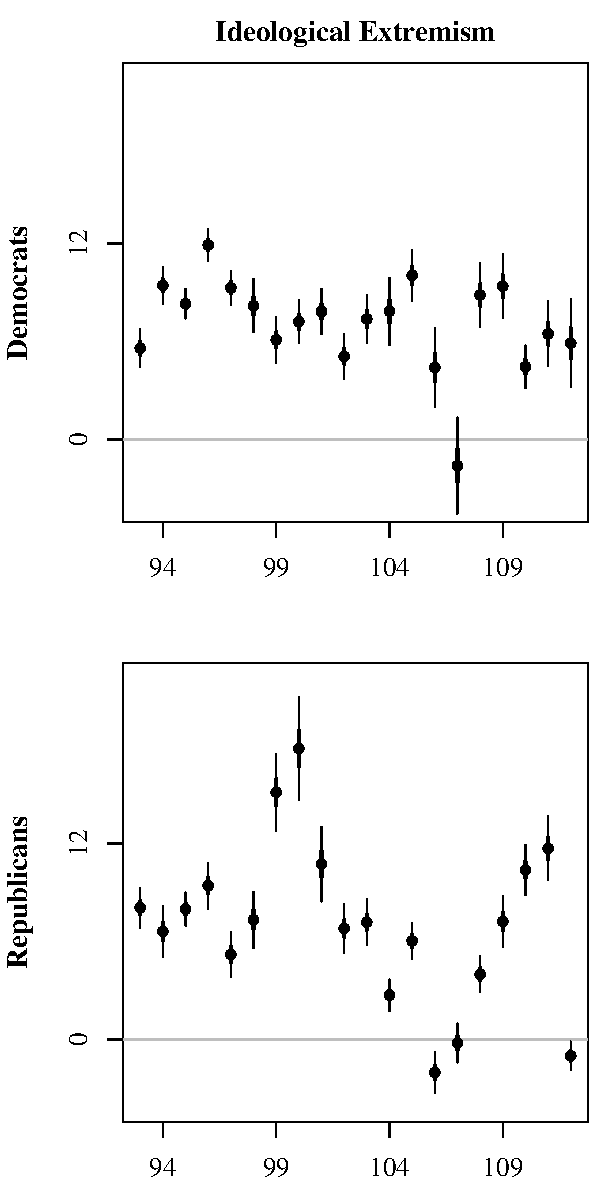
\includegraphics[width = 10cm]{C:/Users/Ethan/Documents/GitHub/partycalls/plots/who-heeds-figure2-interaction_party.pdf}
\end{figure}

\begin{figure}[H]
	\centering
	\caption{House Ideological Extremism Coefficient Plot, Southern and Other Democrats}
	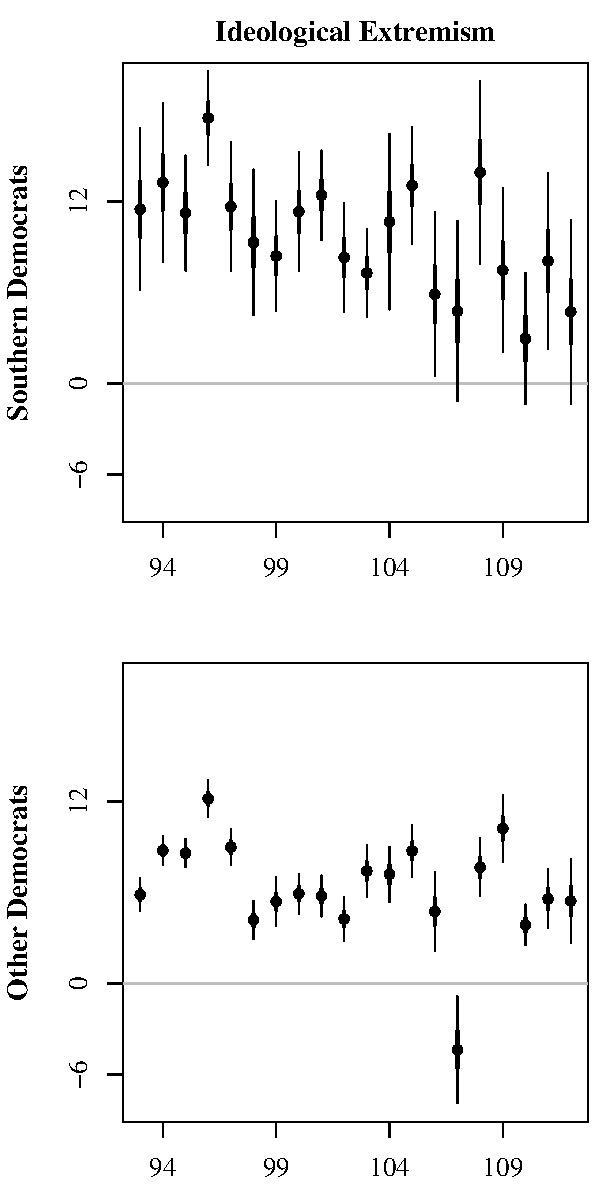
\includegraphics[width = 10cm]{C:/Users/Ethan/Documents/GitHub/partycalls/plots/who-heeds-figure2-interaction-south-other-dems.pdf}
\end{figure}

\begin{figure}[H]
	\centering
	\caption{Senate Ideological Extremism Coefficient Plot, Majority}
	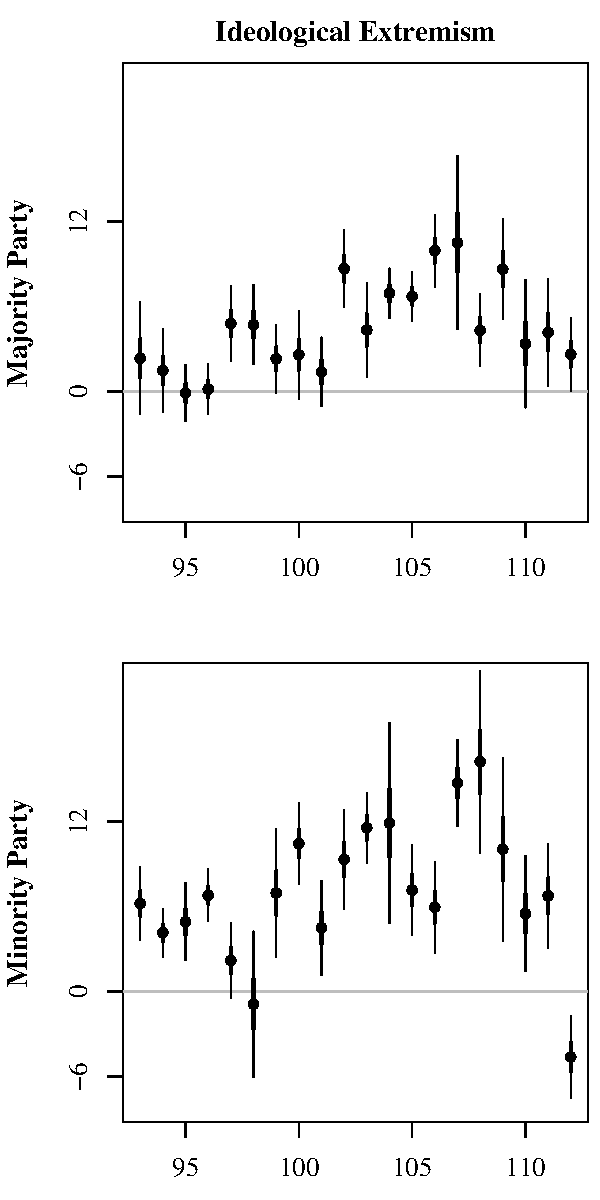
\includegraphics[width = 10cm]{C:/Users/Ethan/Documents/GitHub/partycalls/plots/senate-figure2-interaction.pdf}
\end{figure}

\begin{figure}[H]
	\centering
	\caption{Senate Ideological Extremism Coefficient Plot, Party}
	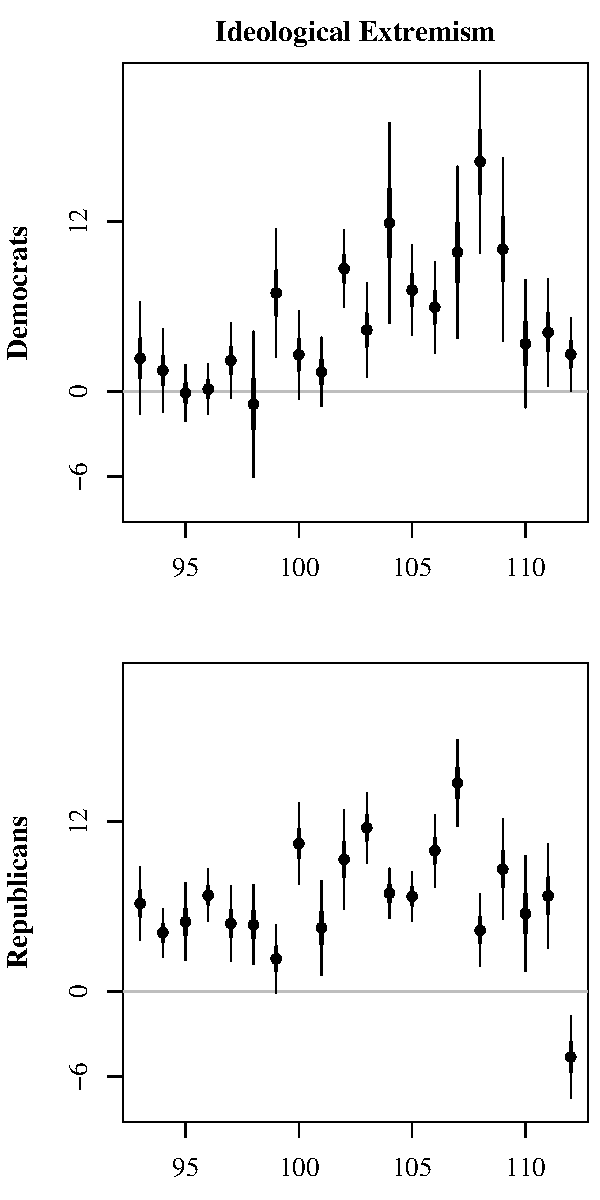
\includegraphics[width = 10cm]{C:/Users/Ethan/Documents/GitHub/partycalls/plots/senate-figure2-interaction-party.pdf}
\end{figure}

\begin{figure}[H]
	\centering
	\caption{Senate Ideological Extremism Coefficient Plot, Election Proximity}
	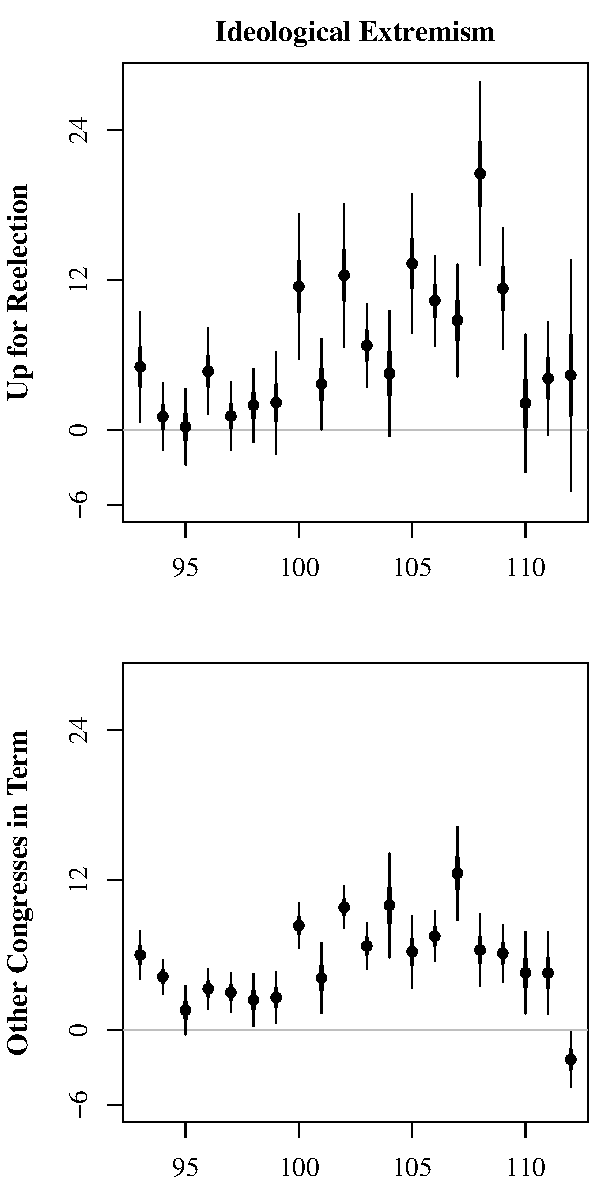
\includegraphics[width = 10cm]{C:/Users/Ethan/Documents/GitHub/partycalls/plots/senate-figure2-interaction-reelection.pdf}
\end{figure}

\begin{figure}[H]
	\centering
	\caption{Senate Ideological Extremism Coefficient Plot, Gingrich Senators and Other Republicans}
	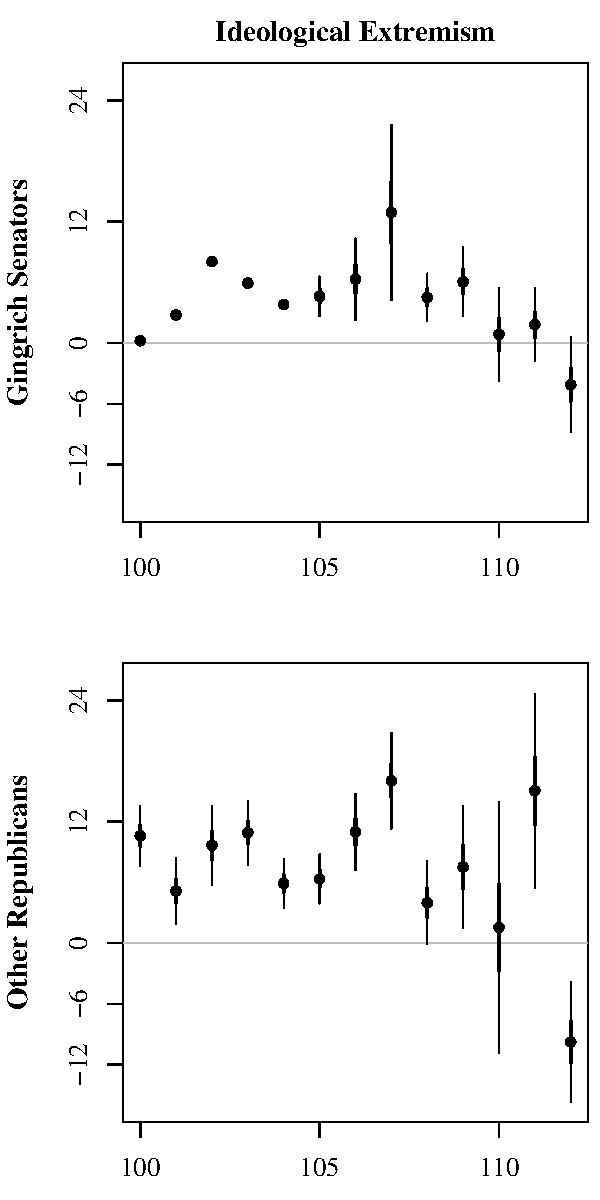
\includegraphics[width = 10cm]{C:/Users/Ethan/Documents/GitHub/partycalls/plots/senate-figure2-interaction-gingrich-other-reps.pdf}
\end{figure}

\begin{figure}[H]
	\centering
	\caption{Senate Ideological Extremism Coefficient Plot, Southern and Other Democrats}
	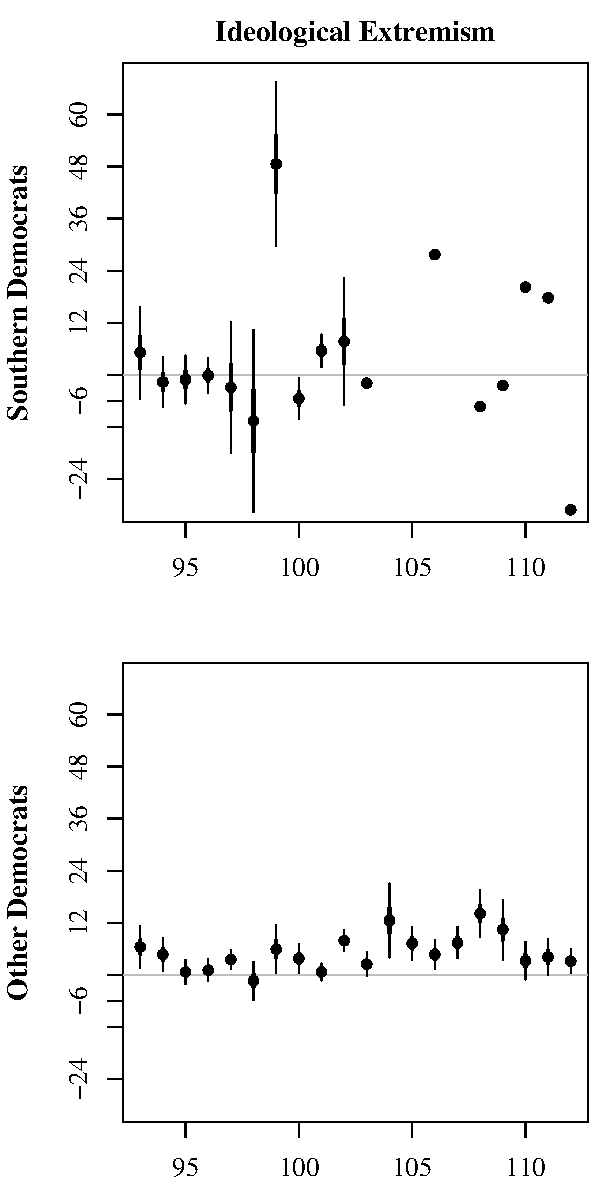
\includegraphics[width = 10cm]{C:/Users/Ethan/Documents/GitHub/partycalls/plots/senate-figure2-interaction-southern-other-dems.pdf}
\end{figure}

\pagebreak

\subsection{Models Without Vote Share Interaction}

\begin{table}[H]
		\begin{center}
			\caption{Senate Inter-Party Regression Models, DV: pirate100}
			\begin{tabular}{l c c c c }
				\hline
				& Democrats & Republicans & Majority & Minority \\
				\hline
				ideological\_extremism & $6.823^{***}$  & $8.655^{***}$   & $8.004^{***}$  & $10.214^{***}$ \\
				& $(0.487)$      & $(0.451)$       & $(0.386)$      & $(0.465)$      \\
				pres\_vote\_share      & $33.909^{***}$ & $-10.484^{**}$  & $20.963^{***}$ & $-1.677$       \\
				& $(3.010)$      & $(3.902)$       & $(2.604)$      & $(3.869)$      \\
				south                  & $-3.170^{***}$ & $2.592^{***}$   & $-1.430^{*}$   & $0.609$        \\
				& $(0.706)$      & $(0.726)$       & $(0.561)$      & $(0.755)$      \\
				vote\_share            & $-7.562^{**}$  & $21.321^{***}$  & $-1.805$       & $10.066^{**}$  \\
				& $(2.750)$      & $(3.534)$       & $(2.734)$      & $(3.590)$      \\
				female                 & $3.661^{***}$  & $-0.412$        & $3.612^{***}$  & $6.439^{***}$  \\
				& $(0.924)$      & $(1.434)$       & $(0.992)$      & $(1.345)$      \\
				afam                   & $-2.333$       & $-24.693^{***}$ & $3.110$        & $-10.298^{**}$ \\
				& $(3.552)$      & $(5.371)$       & $(5.537)$      & $(3.898)$      \\
				latino                 & $6.315^{*}$    & $5.317$         & $6.614^{**}$   & $7.472$        \\
				& $(2.791)$      & $(3.520)$       & $(2.484)$      & $(4.258)$      \\
				up\_for\_reelection    & $-0.483$       & $-0.894$        & $-0.689$       & $-0.994$       \\
				& $(0.542)$      & $(0.681)$       & $(0.544)$      & $(0.732)$      \\
				seniority              & $-0.081$       & $-0.054$        & $0.216^{**}$   & $0.145$        \\
				& $(0.066)$      & $(0.091)$       & $(0.079)$      & $(0.085)$      \\
				freshman               & $1.284$        & $1.425$         & $1.441$        & $1.278$        \\
				& $(0.902)$      & $(1.066)$       & $(0.834)$      & $(1.253)$      \\
				retiree                & $1.399$        & $0.668$         & $0.807$        & $1.698$        \\
				& $(1.142)$      & $(1.260)$       & $(1.125)$      & $(1.347)$      \\
				best\_committee        & $0.367^{*}$    & $-0.411^{*}$    & $0.010$        & $0.062$        \\
				& $(0.158)$      & $(0.194)$       & $(0.156)$      & $(0.211)$      \\
				leader                 & $3.322^{***}$  & $3.113^{**}$    & $2.275^{**}$   & $3.336^{**}$   \\
				& $(0.906)$      & $(0.976)$       & $(0.874)$      & $(1.088)$      \\
				power\_committee       & $0.202$        & $1.321$         & $1.323$        & $-0.339$       \\
				& $(0.982)$      & $(1.168)$       & $(0.950)$      & $(1.290)$      \\
				chair                  & $1.989^{**}$   & $4.842^{***}$   & $-1.149$       &                \\
				& $(0.690)$      & $(0.885)$       & $(0.682)$      &                \\
				(Intercept)            & $65.124^{***}$ & $74.581^{***}$  & $70.354^{***}$ & $67.835^{***}$ \\
				& $(2.420)$      & $(3.247)$       & $(2.387)$      & $(3.396)$      \\
				\hline
				R$^2$                  & 0.495          & 0.424           & 0.446          & 0.431          \\
				Adj. R$^2$             & 0.487          & 0.414           & 0.438          & 0.421          \\
				Num. obs.              & 1042           & 951             & 1052           & 843            \\
				RMSE                   & 7.795          & 9.192           & 7.762          & 9.411          \\
				\hline
				\multicolumn{5}{l}{\scriptsize{$^{***}p<0.001$, $^{**}p<0.01$, $^*p<0.05$}}
			\end{tabular}
		\end{center}
\end{table}

\begin{table}[H]
	\begin{center}
		\caption{Senate Intra-Party Regression, DV: pirate100}
		\begin{tabular}{l c c c c }
			\hline
			& \multicolumn{2}{c}{Democrats} & \multicolumn{2}{c}{Republicans} \\
			\cline{2-5}
			& Southern & Others & Gingrich Senators & Others \\
			\hline
			ideological\_extremism & $12.327^{***}$ & $4.642^{***}$  & $1.840^{**}$   & $8.372^{***}$   \\
			& $(1.303)$      & $(0.471)$      & $(0.635)$      & $(0.528)$       \\
			pres\_vote\_share      & $32.062^{***}$ & $32.871^{***}$ & $6.642$        & $-5.847$        \\
			& $(6.694)$      & $(3.090)$      & $(4.726)$      & $(4.593)$       \\
			latino                 &                & $6.777^{**}$   & $0.509$        & $4.051$         \\
			&                & $(2.338)$      & $(2.627)$      & $(4.844)$       \\
			vote\_share            & $-7.161$       & $-0.618$       & $1.793$        & $19.594^{***}$  \\
			& $(4.874)$      & $(3.374)$      & $(3.726)$      & $(4.266)$       \\
			female                 & $2.722$        & $4.003^{***}$  &                & $1.115$         \\
			& $(2.607)$      & $(0.872)$      &                & $(1.501)$       \\
			up\_for\_reelection    & $-1.765$       & $-0.176$       & $-0.077$       & $-1.439$        \\
			& $(1.413)$      & $(0.516)$      & $(0.737)$      & $(0.785)$       \\
			seniority              & $-0.701^{***}$ & $0.066$        & $-0.473^{*}$   & $0.109$         \\
			& $(0.180)$      & $(0.065)$      & $(0.184)$      & $(0.101)$       \\
			freshman               & $2.647$        & $1.035$        & $-0.733$       & $1.380$         \\
			& $(2.329)$      & $(0.866)$      & $(1.021)$      & $(1.296)$       \\
			retiree                & $3.421$        & $1.813$        & $2.025$        & $0.744$         \\
			& $(2.966)$      & $(1.105)$      & $(1.702)$      & $(1.403)$       \\
			best\_committee        & $0.793$        & $0.243$        & $-0.083$       & $-0.327$        \\
			& $(0.404)$      & $(0.154)$      & $(0.190)$      & $(0.237)$       \\
			leader                 & $5.668$        & $2.775^{***}$  & $3.039^{*}$    & $2.860^{*}$     \\
			& $(3.040)$      & $(0.827)$      & $(1.171)$      & $(1.117)$       \\
			power\_committee       & $2.598$        & $-1.180$       & $1.983$        & $0.118$         \\
			& $(2.770)$      & $(0.931)$      & $(1.173)$      & $(1.417)$       \\
			chair                  & $3.745^{*}$    & $1.974^{**}$   & $0.809$        & $5.506^{***}$   \\
			& $(1.844)$      & $(0.657)$      & $(1.178)$      & $(0.985)$       \\
			afam                   &                & $-1.649$       &                & $-22.812^{***}$ \\
			&                & $(2.980)$      &                & $(5.563)$       \\
			south                  &                &                & $0.262$        & $2.961^{***}$   \\
			&                &                & $(0.750)$      & $(0.880)$       \\
			(Intercept)            & $59.038^{***}$ & $64.692^{***}$ & $87.816^{***}$ & $70.926^{***}$  \\
			& $(5.690)$      & $(2.481)$      & $(3.073)$      & $(3.953)$       \\
			\hline
			R$^2$                  & 0.526          & 0.387          & 0.132          & 0.420           \\
			Adj. R$^2$             & 0.501          & 0.376          & 0.067          & 0.408           \\
			Num. obs.              & 246            & 796            & 188            & 763             \\
			RMSE                   & 9.664          & 6.508          & 4.323          & 9.506           \\
			\hline
			\multicolumn{5}{l}{\scriptsize{$^{***}p<0.001$, $^{**}p<0.01$, $^*p<0.05$}}
		\end{tabular}
	\end{center}
\end{table}

\begin{table}[H]
	\begin{center}
		\caption{Senate Inter-Party Fixed Effects Models, DV: pirate100}
		\begin{tabular}{l c c c c }
			\hline
			& Democrats & Republicans & Majority & Minority \\
			\hline
			ideological\_extremism  & $4.37^{***}$  & $4.08^{***}$  & $2.89^{**}$   & $4.03^{***}$ \\
			& $(0.89)$      & $(0.97)$      & $(0.89)$      & $(1.08)$     \\
			vote\_share             & $3.21$        & $-5.73^{*}$   & $2.88$        & $-2.02$      \\
			& $(2.65)$      & $(2.88)$      & $(3.44)$      & $(3.53)$     \\
			pres\_vote\_share       & $31.19^{***}$ & $7.90$        & $33.44^{***}$ & $15.00^{*}$  \\
			& $(5.36)$      & $(6.19)$      & $(7.17)$      & $(6.34)$     \\
			freshman                & $0.67$        & $1.14^{*}$    & $1.01^{*}$    & $0.94$       \\
			& $(0.51)$      & $(0.49)$      & $(0.48)$      & $(0.77)$     \\
			retiree                 & $0.12$        & $0.70$        & $0.18$        & $0.77$       \\
			& $(0.91)$      & $(0.89)$      & $(1.10)$      & $(0.96)$     \\
			best\_committee         & $0.13$        & $0.10$        & $0.34^{*}$    & $0.31$       \\
			& $(0.14)$      & $(0.17)$      & $(0.16)$      & $(0.18)$     \\
			up\_for\_reelection     & $-0.45$       & $-1.44^{***}$ & $-0.79^{*}$   & $-1.02^{**}$ \\
			& $(0.30)$      & $(0.35)$      & $(0.32)$      & $(0.36)$     \\
			power\_committee        & $-0.59$       & $-0.01$       & $-1.52$       & $-0.16$      \\
			& $(0.82)$      & $(1.06)$      & $(1.03)$      & $(1.03)$     \\
			leader                  & $1.24^{*}$    & $1.60^{*}$    & $1.55$        & $1.46$       \\
			& $(0.61)$      & $(0.66)$      & $(0.85)$      & $(0.87)$     \\
			chair                   & $0.58$        & $0.74$        & $-0.67$       &              \\
			& $(0.65)$      & $(0.76)$      & $(0.60)$      &              \\
			\hline
			Num. obs.               & 1042          & 951           & 1052          & 843          \\
			R$^2$      & 0.17          & 0.13          & 0.18          & 0.14         \\
			Adj. R$^2$ & 0.85          & 0.87          & 0.87          & 0.90         \\
			\hline
			\multicolumn{5}{l}{\scriptsize{$^{***}p<0.001$, $^{**}p<0.01$, $^*p<0.05$}}
		\end{tabular}
	\end{center}
\end{table}

\begin{table}[H]
	\begin{center}
		\caption{Senate Intra-Party Fixed Effects Models, DV: pirate100}
		\begin{tabular}{l c c c c }
			\hline
			& \multicolumn{2}{c}{Democrats} & \multicolumn{2}{c}{Republicans} \\
			\cline{2-5}
			& Southern & Others & Gingrich Senators & Others \\
			\hline
			ideological\_extremism  & $11.34^{***}$ & $2.92^{***}$ & $1.78$   & $4.31^{***}$  \\
			& $(1.76)$      & $(0.87)$     & $(1.54)$ & $(1.17)$      \\
			vote\_share             & $1.40$        & $5.89$       & $-0.99$  & $-6.61$       \\
			& $(3.37)$      & $(3.65)$     & $(3.95)$ & $(3.52)$      \\
			pres\_vote\_share       & $22.41^{*}$   & $12.47$      & $2.51$   & $8.91$        \\
			& $(11.01)$     & $(7.05)$     & $(9.16)$ & $(6.96)$      \\
			freshman                & $0.76$        & $1.04^{*}$   & $-0.55$  & $1.89^{**}$   \\
			& $(0.85)$      & $(0.53)$     & $(0.73)$ & $(0.60)$      \\
			retiree                 & $-2.92$       & $0.88$       & $1.20$   & $0.60$        \\
			& $(2.06)$      & $(0.69)$     & $(1.16)$ & $(1.02)$      \\
			best\_committee         & $0.48$        & $0.03$       & $0.26$   & $0.04$        \\
			& $(0.31)$      & $(0.13)$     & $(0.27)$ & $(0.22)$      \\
			up\_for\_reelection     & $-0.40$       & $-0.36$      & $-0.45$  & $-1.75^{***}$ \\
			& $(0.71)$      & $(0.32)$     & $(0.60)$ & $(0.40)$      \\
			power\_committee        & $-2.19$       & $-0.10$      & $-0.57$  & $0.39$        \\
			& $(2.22)$      & $(0.77)$     & $(1.10)$ & $(1.28)$      \\
			leader                  & $2.73$        & $1.30^{*}$   & $1.22$   & $1.64^{*}$    \\
			& $(2.33)$      & $(0.54)$     & $(0.85)$ & $(0.79)$      \\
			chair                   & $1.81$        & $0.38$       & $-1.32$  & $0.92$        \\
			& $(1.50)$      & $(0.60)$     & $(0.76)$ & $(0.91)$      \\
			\hline
			Num. obs.               & 246           & 796          & 188      & 763           \\
			R$^2$     & 0.91          & 0.85         & 0.65     & 0.90          \\
			Adj. R$^2$ & 0.87          & 0.81         & 0.49     & 0.87          \\
			\hline
			\multicolumn{5}{l}{\scriptsize{$^{***}p<0.001$, $^{**}p<0.01$, $^*p<0.05$}}
		\end{tabular}
	\end{center}
\end{table}

\begin{table}[H]
	\begin{center}
		\caption{Senate Inter-Party Regression Models, DV: pfrate100}
		\begin{tabular}{l c c c c }
			\hline
			& Democrats & Republicans & Majority & Minority \\
			\hline
			ideological\_extremism & $4.857^{***}$  & $1.163^{**}$    & $4.695^{***}$  & $3.226^{***}$  \\
			& $(0.398)$      & $(0.373)$       & $(0.361)$      & $(0.377)$      \\
			pres\_vote\_share      & $13.872^{***}$ & $3.896$         & $3.918$        & $-3.194$       \\
			& $(2.459)$      & $(3.235)$       & $(2.431)$      & $(3.131)$      \\
			south                  & $-1.949^{***}$ & $2.320^{***}$   & $-2.114^{***}$ & $-0.677$       \\
			& $(0.577)$      & $(0.602)$       & $(0.524)$      & $(0.611)$      \\
			vote\_share            & $-3.036$       & $8.640^{**}$    & $-0.894$       & $3.513$        \\
			& $(2.247)$      & $(2.929)$       & $(2.554)$      & $(2.905)$      \\
			female                 & $2.597^{***}$  & $-1.164$        & $4.387^{***}$  & $3.109^{**}$   \\
			& $(0.755)$      & $(1.188)$       & $(0.926)$      & $(1.089)$      \\
			afam                   & $-1.540$       & $-18.748^{***}$ & $2.249$        & $-6.806^{*}$   \\
			& $(2.902)$      & $(4.451)$       & $(5.170)$      & $(3.155)$      \\
			latino                 & $5.929^{**}$   & $-2.624$        & $2.611$        & $1.737$        \\
			& $(2.280)$      & $(2.917)$       & $(2.320)$      & $(3.445)$      \\
			up\_for\_reelection    & $0.195$        & $0.732$         & $0.374$        & $0.300$        \\
			& $(0.443)$      & $(0.564)$       & $(0.508)$      & $(0.592)$      \\
			seniority              & $-0.161^{**}$  & $-0.040$        & $0.197^{**}$   & $0.039$        \\
			& $(0.054)$      & $(0.076)$       & $(0.074)$      & $(0.068)$      \\
			freshman               & $0.679$        & $1.439$         & $1.197$        & $0.402$        \\
			& $(0.737)$      & $(0.883)$       & $(0.779)$      & $(1.014)$      \\
			retiree                & $-0.264$       & $-2.188^{*}$    & $-1.436$       & $-1.249$       \\
			& $(0.933)$      & $(1.045)$       & $(1.050)$      & $(1.090)$      \\
			best\_committee        & $0.171$        & $-0.565^{***}$  & $-0.023$       & $-0.444^{**}$  \\
			& $(0.129)$      & $(0.161)$       & $(0.146)$      & $(0.171)$      \\
			leader                 & $1.455^{*}$    & $2.971^{***}$   & $1.189$        & $1.988^{*}$    \\
			& $(0.740)$      & $(0.809)$       & $(0.816)$      & $(0.881)$      \\
			power\_committee       & $1.392$        & $2.220^{*}$     & $1.959^{*}$    & $1.607$        \\
			& $(0.802)$      & $(0.968)$       & $(0.887)$      & $(1.044)$      \\
			chair                  & $1.499^{**}$   & $1.640^{*}$     & $-1.612^{*}$   &                \\
			& $(0.563)$      & $(0.734)$       & $(0.637)$      &                \\
			(Intercept)            & $73.355^{***}$ & $76.051^{***}$  & $76.913^{***}$ & $81.225^{***}$ \\
			& $(1.977)$      & $(2.691)$       & $(2.229)$      & $(2.748)$      \\
			\hline
			R$^2$                  & 0.353          & 0.123           & 0.233          & 0.124          \\
			Adj. R$^2$             & 0.344          & 0.109           & 0.222          & 0.109          \\
			Num. obs.              & 1042           & 951             & 1052           & 843            \\
			RMSE                   & 6.368          & 7.619           & 7.249          & 7.616          \\
			\hline
			\multicolumn{5}{l}{\scriptsize{$^{***}p<0.001$, $^{**}p<0.01$, $^*p<0.05$}}
		\end{tabular}
	\end{center}
\end{table}

\begin{table}[H]
	\begin{center}
		\caption{Senate Intra-Party Regression, DV: pfrate100}
		\begin{tabular}{l c c c c }
			\hline
			& \multicolumn{2}{c}{Democrats} & \multicolumn{2}{c}{Republicans} \\
			\cline{2-5}
			& Southern & Others & Gingrich Senators & Others \\
			\hline
			ideological\_extremism & $9.181^{***}$  & $3.176^{***}$  & $-4.803^{***}$ & $2.234^{***}$   \\
			& $(1.000)$      & $(0.407)$      & $(0.902)$      & $(0.426)$       \\
			pres\_vote\_share      & $6.294$        & $15.590^{***}$ & $24.864^{***}$ & $-0.677$        \\
			& $(5.140)$      & $(2.673)$      & $(6.709)$      & $(3.705)$       \\
			latino                 &                & $6.314^{**}$   & $-9.826^{**}$  & $0.765$         \\
			&                & $(2.022)$      & $(3.729)$      & $(3.908)$       \\
			vote\_share            & $-5.155$       & $4.284$        & $-2.390$       & $12.163^{***}$  \\
			& $(3.743)$      & $(2.919)$      & $(5.290)$      & $(3.442)$       \\
			female                 & $2.948$        & $2.408^{**}$   &                & $-0.975$        \\
			& $(2.002)$      & $(0.755)$      &                & $(1.211)$       \\
			up\_for\_reelection    & $-0.255$       & $0.263$        & $1.593$        & $0.419$         \\
			& $(1.085)$      & $(0.446)$      & $(1.046)$      & $(0.633)$       \\
			seniority              & $-0.478^{***}$ & $-0.110$       & $-0.857^{**}$  & $-0.036$        \\
			& $(0.138)$      & $(0.056)$      & $(0.261)$      & $(0.082)$       \\
			freshman               & $0.717$        & $0.529$        & $-2.195$       & $1.500$         \\
			& $(1.789)$      & $(0.750)$      & $(1.450)$      & $(1.045)$       \\
			retiree                & $2.079$        & $-0.193$       & $-3.221$       & $-2.011$        \\
			& $(2.277)$      & $(0.956)$      & $(2.415)$      & $(1.132)$       \\
			best\_committee        & $0.257$        & $0.175$        & $-0.674^{*}$   & $-0.449^{*}$    \\
			& $(0.310)$      & $(0.133)$      & $(0.270)$      & $(0.191)$       \\
			leader                 & $-0.102$       & $1.551^{*}$    & $4.697^{**}$   & $2.292^{*}$     \\
			& $(2.334)$      & $(0.715)$      & $(1.662)$      & $(0.901)$       \\
			power\_committee       & $2.205$        & $0.284$        & $3.719^{*}$    & $1.646$         \\
			& $(2.127)$      & $(0.806)$      & $(1.665)$      & $(1.143)$       \\
			chair                  & $0.766$        & $2.197^{***}$  & $-1.974$       & $2.197^{**}$    \\
			& $(1.416)$      & $(0.569)$      & $(1.672)$      & $(0.795)$       \\
			afam                   &                & $-1.005$       &                & $-18.074^{***}$ \\
			&                & $(2.578)$      &                & $(4.488)$       \\
			south                  &                &                & $0.992$        & $2.359^{***}$   \\
			&                &                & $(1.064)$      & $(0.710)$       \\
			(Intercept)            & $76.810^{***}$ & $69.742^{***}$ & $82.148^{***}$ & $75.029^{***}$  \\
			& $(4.369)$      & $(2.147)$      & $(4.362)$      & $(3.189)$       \\
			\hline
			R$^2$                  & 0.455          & 0.223          & 0.313          & 0.161           \\
			Adj. R$^2$             & 0.427          & 0.209          & 0.261          & 0.144           \\
			Num. obs.              & 246            & 796            & 188            & 763             \\
			RMSE                   & 7.421          & 5.630          & 6.137          & 7.669           \\
			\hline
			\multicolumn{5}{l}{\scriptsize{$^{***}p<0.001$, $^{**}p<0.01$, $^*p<0.05$}}
		\end{tabular}
	\end{center}
\end{table}

\begin{table}[H]
	\begin{center}
		\caption{Senate Inter-Party Fixed Effects Models, DV: pfrate100}
		\begin{tabular}{l c c c c }
			\hline
			& Democrats & Republicans & Majority & Minority \\
			\hline
			ideological\_extremism  & $4.01^{***}$ & $0.34$   & $2.95^{*}$ & $0.54$   \\
			& $(1.19)$     & $(1.51)$ & $(1.21)$   & $(1.42)$ \\
			vote\_share             & $1.86$       & $-1.25$  & $1.64$     & $0.21$   \\
			& $(3.39)$     & $(3.73)$ & $(4.55)$   & $(3.86)$ \\
			pres\_vote\_share       & $10.07$      & $-3.02$  & $7.55$     & $6.13$   \\
			& $(5.76)$     & $(7.31)$ & $(5.84)$   & $(7.52)$ \\
			freshman                & $-0.10$      & $0.64$   & $0.66$     & $0.92$   \\
			& $(0.50)$     & $(0.63)$ & $(0.53)$   & $(0.95)$ \\
			retiree                 & $-0.33$      & $-0.75$  & $-0.50$    & $0.12$   \\
			& $(0.76)$     & $(0.99)$ & $(1.08)$   & $(1.13)$ \\
			best\_committee         & $-0.04$      & $-0.03$  & $0.14$     & $-0.32$  \\
			& $(0.13)$     & $(0.21)$ & $(0.17)$   & $(0.21)$ \\
			up\_for\_reelection     & $0.26$       & $0.45$   & $0.63$     & $0.13$   \\
			& $(0.33)$     & $(0.32)$ & $(0.34)$   & $(0.42)$ \\
			power\_committee        & $-0.29$      & $0.83$   & $-0.72$    & $1.63$   \\
			& $(0.94)$     & $(1.12)$ & $(1.13)$   & $(1.02)$ \\
			leader                  & $1.01$       & $0.57$   & $0.44$     & $0.88$   \\
			& $(0.97)$     & $(0.55)$ & $(0.89)$   & $(1.04)$ \\
			chair                   & $0.53$       & $0.37$   & $-0.29$    &          \\
			& $(0.61)$     & $(0.85)$ & $(0.73)$   &          \\
			\hline
			Num. obs.               & 1042         & 951      & 1052       & 843      \\
			R$^2$      & 0.82         & 0.74     & 0.83       & 0.81     \\
			Adj. R$^2$ & 0.77         & 0.68     & 0.76       & 0.73     \\
			\hline
			\multicolumn{5}{l}{\scriptsize{$^{***}p<0.001$, $^{**}p<0.01$, $^*p<0.05$}}
		\end{tabular}
	\end{center}
\end{table}

\begin{table}[H]
	\begin{center}
		\caption{Senate Intra-Party Fixed Effects Models, DV: pfrate100}
		\begin{tabular}{l c c c c }
			\hline
			& \multicolumn{2}{c}{Democrats} & \multicolumn{2}{c}{Republicans} \\
			\cline{2-5}
			& Southern & Others & Gingrich Senators & Others \\
			\hline
			ideological\_extremism  & $10.52^{***}$ & $2.33^{*}$ & $-2.90$    & $1.11$   \\
			& $(1.76)$      & $(1.17)$   & $(2.54)$   & $(1.81)$ \\
			vote\_share             & $1.59$        & $1.93$     & $-2.20$    & $0.65$   \\
			& $(2.58)$      & $(3.50)$   & $(6.76)$   & $(3.57)$ \\
			pres\_vote\_share       & $14.66$       & $-0.70$    & $20.94$    & $-7.71$  \\
			& $(9.87)$      & $(7.53)$   & $(18.26)$  & $(7.22)$ \\
			freshman                & $-0.17$       & $-0.06$    & $-1.27$    & $1.31$   \\
			& $(0.96)$      & $(0.53)$   & $(1.36)$   & $(0.67)$ \\
			retiree                 & $-0.81$       & $0.03$     & $-1.87$    & $-0.62$  \\
			& $(1.37)$      & $(0.77)$   & $(3.27)$   & $(1.03)$ \\
			best\_committee         & $-0.05$       & $-0.02$    & $-0.21$    & $-0.06$  \\
			& $(0.17)$      & $(0.13)$   & $(0.48)$   & $(0.24)$ \\
			up\_for\_reelection     & $0.38$        & $0.24$     & $1.74^{*}$ & $0.24$   \\
			& $(0.49)$      & $(0.40)$   & $(0.67)$   & $(0.35)$ \\
			power\_committee        & $-1.56$       & $0.01$     & $2.35$     & $0.98$   \\
			& $(0.82)$      & $(0.74)$   & $(2.95)$   & $(1.08)$ \\
			leader                  & $0.06$        & $1.37$     & $1.80$     & $0.47$   \\
			& $(1.87)$      & $(0.94)$   & $(1.10)$   & $(0.58)$ \\
			chair                   & $0.91$        & $0.23$     & $-1.41$    & $0.62$   \\
			& $(1.24)$      & $(0.48)$   & $(4.21)$   & $(0.79)$ \\
			\hline
			Num. obs.               & 246           & 796        & 188        & 763      \\
			R$^2$      & 0.92          & 0.75       & 0.68       & 0.78     \\
			Adj. R$^2$ & 0.89          & 0.69       & 0.53       & 0.72     \\
			\hline
			\multicolumn{5}{l}{\scriptsize{$^{***}p<0.001$, $^{**}p<0.01$, $^*p<0.05$}}
		\end{tabular}
	\end{center}
\end{table}

\pagebreak

\subsection{DV/IV and IV/IV Plots With Confidence Bands}

\begin{figure}[H]
	\centering
	\caption{Senate IV/IV Plot, Democrats, Majority Status}
	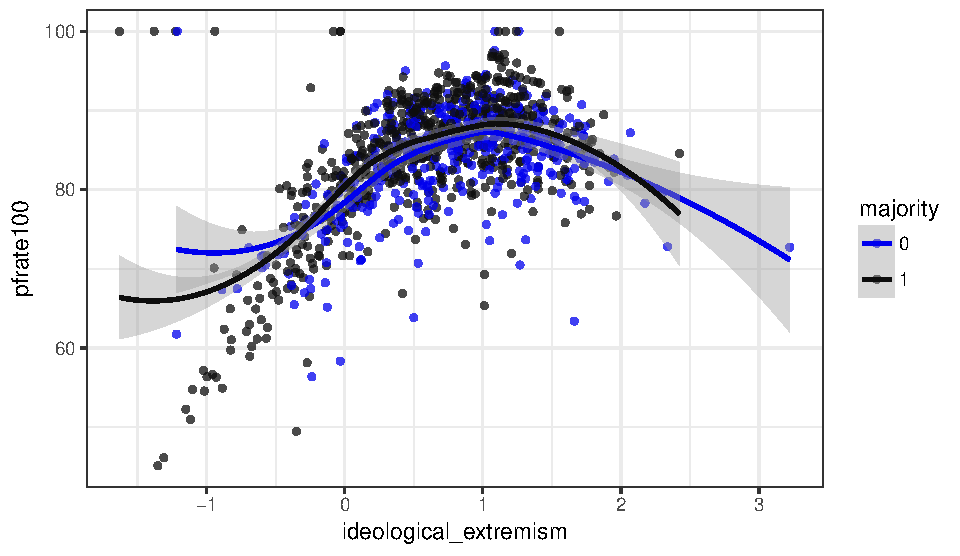
\includegraphics[width = \textwidth]{C:/Users/Ethan/Documents/GitHub/partycalls/plots/senate_dem_iv-iv_majority_confint.pdf}
\end{figure}

\begin{figure}[H]
	\centering
	\caption{Senate DV/IV Plot, Democrats, Majority Status}
	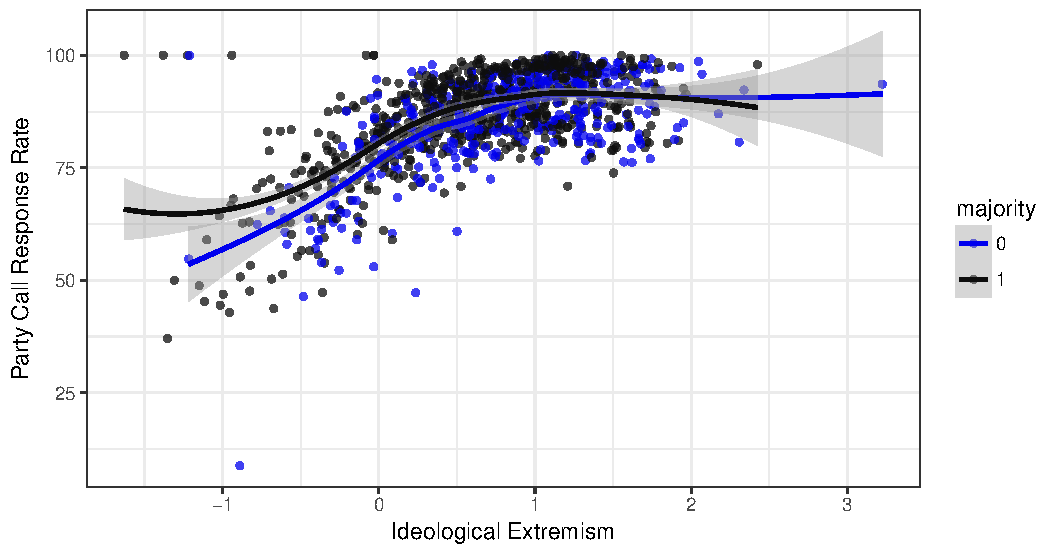
\includegraphics[width = \textwidth]{C:/Users/Ethan/Documents/GitHub/partycalls/plots/senate_dem_iv-dv_majority_confint.pdf}
\end{figure}

\begin{figure}[H]
	\centering
	\caption{Senate IV/IV Plot, Democrats, South/Other}
	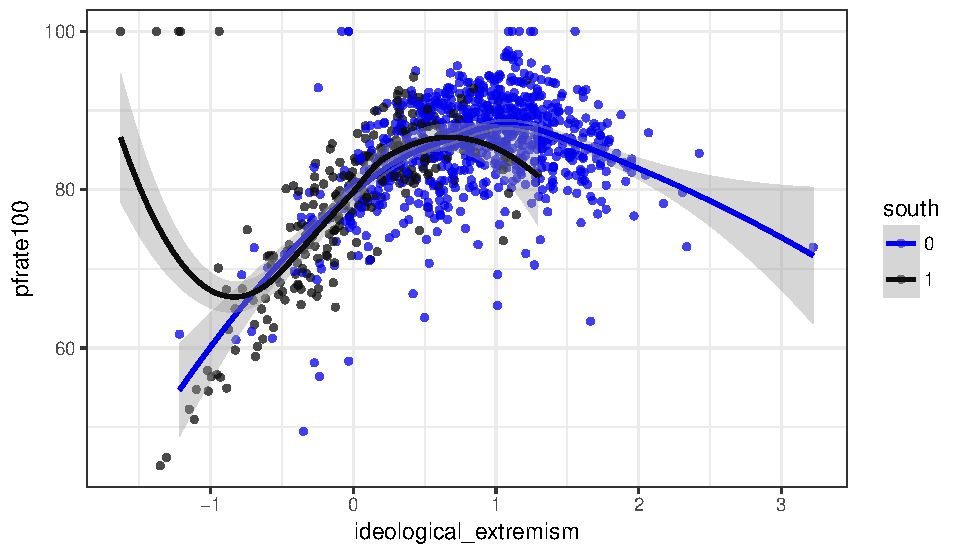
\includegraphics[width = \textwidth]{C:/Users/Ethan/Documents/GitHub/partycalls/plots/senate_dem_iv-iv_south_confint.pdf}
\end{figure}

\begin{figure}[H]
	\centering
	\caption{Senate DV/IV Plot, Democrats, South/Other}
	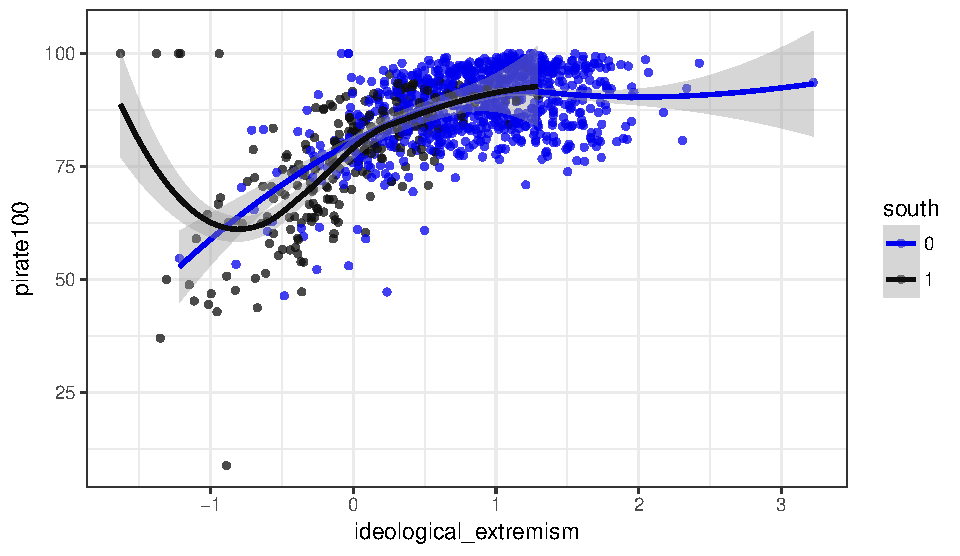
\includegraphics[width = \textwidth]{C:/Users/Ethan/Documents/GitHub/partycalls/plots/senate_dem_iv-dv_south_confint.pdf}
\end{figure}

\begin{figure}[H]
	\centering
	\caption{Senate IV/IV Plot, Republicans, Majority Status}
	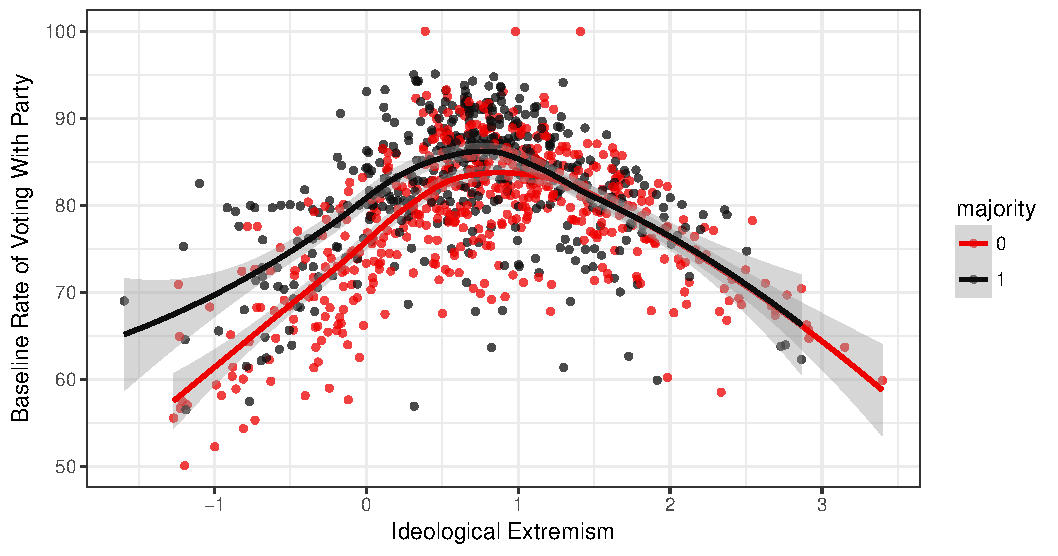
\includegraphics[width = \textwidth]{C:/Users/Ethan/Documents/GitHub/partycalls/plots/senate_rep_iv-iv_majority_confint.pdf}
\end{figure}

\begin{figure}[H]
	\centering
	\caption{Senate DV/IV Plot, Republicans, Majority Status}
	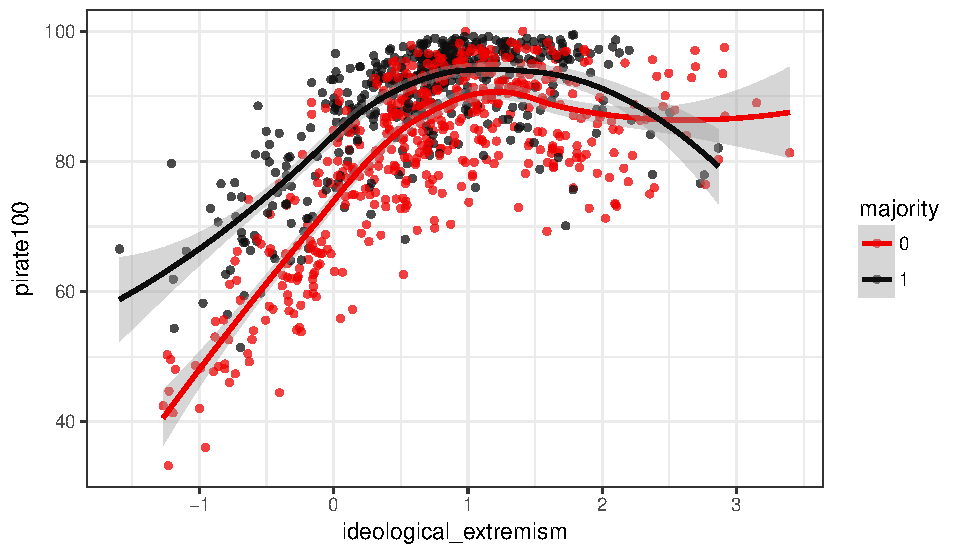
\includegraphics[width = \textwidth]{C:/Users/Ethan/Documents/GitHub/partycalls/plots/senate_rep_iv-dv_majority_confint.pdf}
\end{figure}

\begin{figure}[H]
	\centering
	\caption{Senate IV/IV Plot, Republicans, Gingrich/Other}
	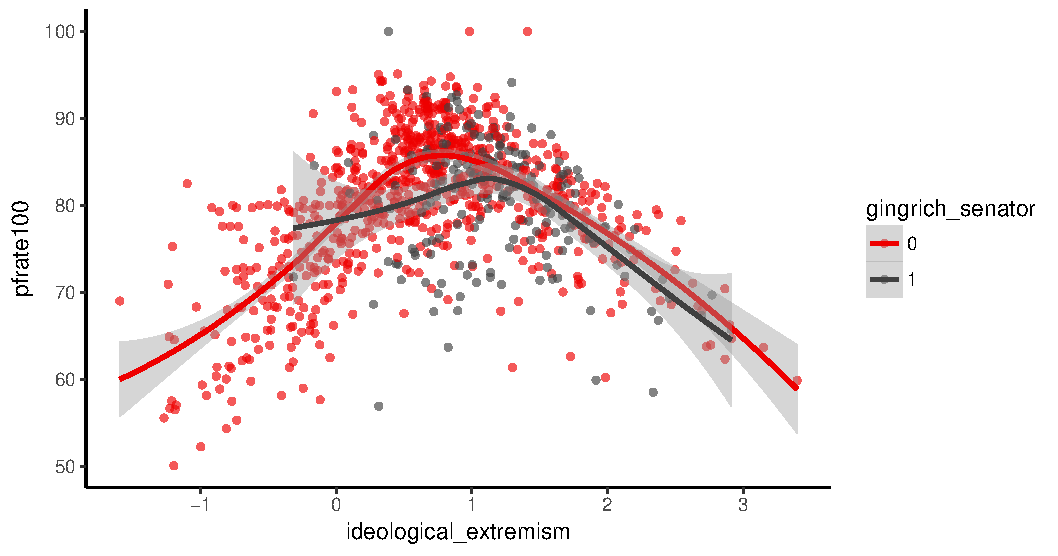
\includegraphics[width = \textwidth]{C:/Users/Ethan/Documents/GitHub/partycalls/plots/senate_rep_iv-iv_gingrich_confint.pdf}
\end{figure}

\begin{figure}[H]
	\centering
	\caption{Senate DV/IV Plot, Republicans, Gingrich/Other}
	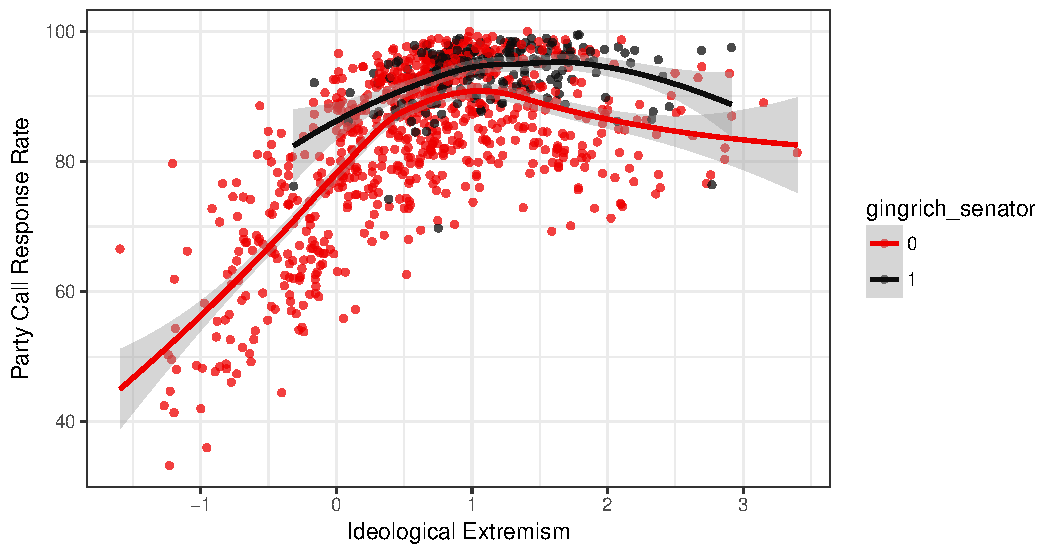
\includegraphics[width = \textwidth]{C:/Users/Ethan/Documents/GitHub/partycalls/plots/senate_rep_iv-dv_gingrich_confint.pdf}
\end{figure}

\begin{figure}[H]
	\centering
	\caption{House IV/IV Plot, Democrats, Majority Status}
	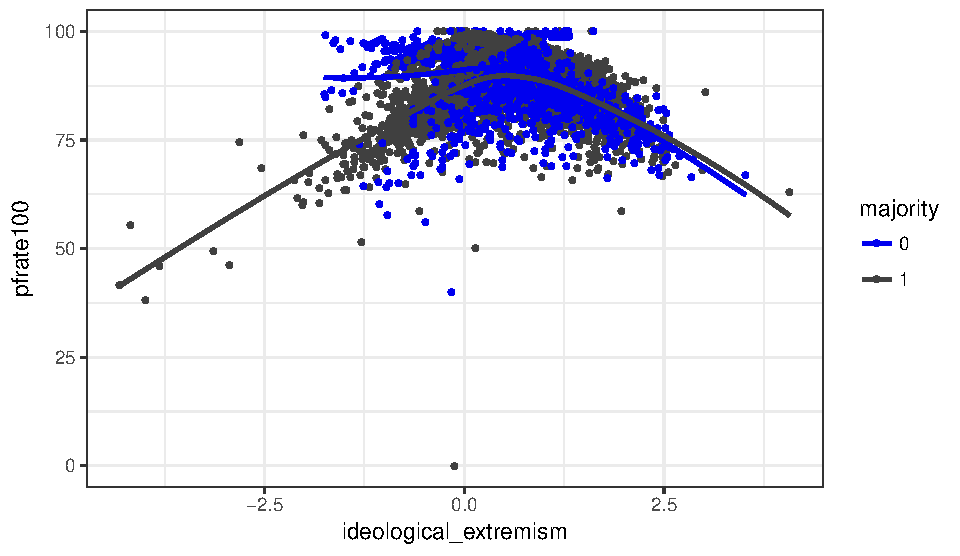
\includegraphics[width = \textwidth]{C:/Users/Ethan/Documents/GitHub/partycalls/plots/house_dem_iv-iv_majority_confint.pdf}
\end{figure}

\begin{figure}[H]
	\centering
	\caption{House DV/IV Plot, Democrats, Majority Status}
	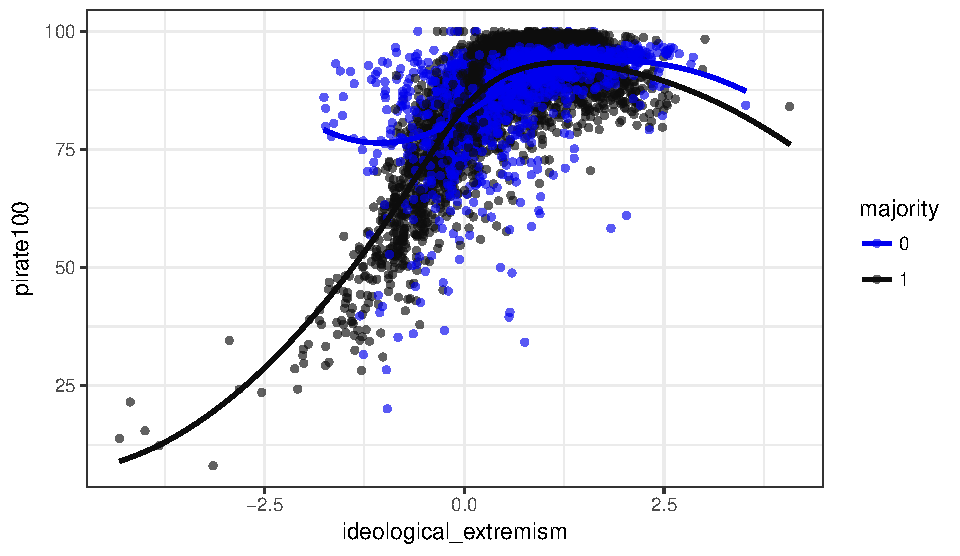
\includegraphics[width = \textwidth]{C:/Users/Ethan/Documents/GitHub/partycalls/plots/house_dem_iv-dv_majority_confint.pdf}
\end{figure}

\begin{figure}[H]
	\centering
	\caption{House IV/IV Plot, Democrats, South/Other}
	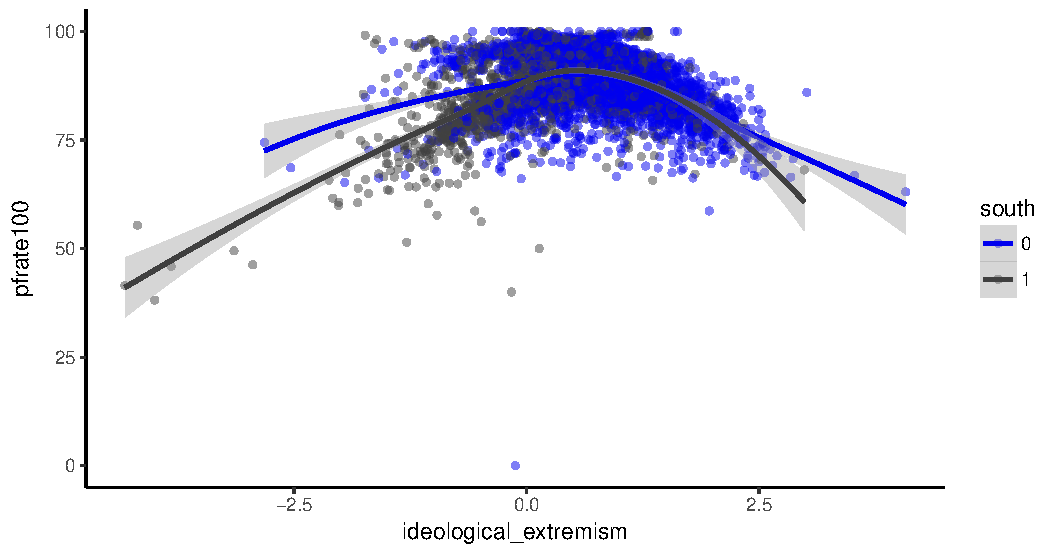
\includegraphics[width = \textwidth]{C:/Users/Ethan/Documents/GitHub/partycalls/plots/house_dem_iv-iv_south_confint.pdf}
\end{figure}

\begin{figure}[H]
	\centering
	\caption{House DV/IV Plot, Democrats, South/Other}
	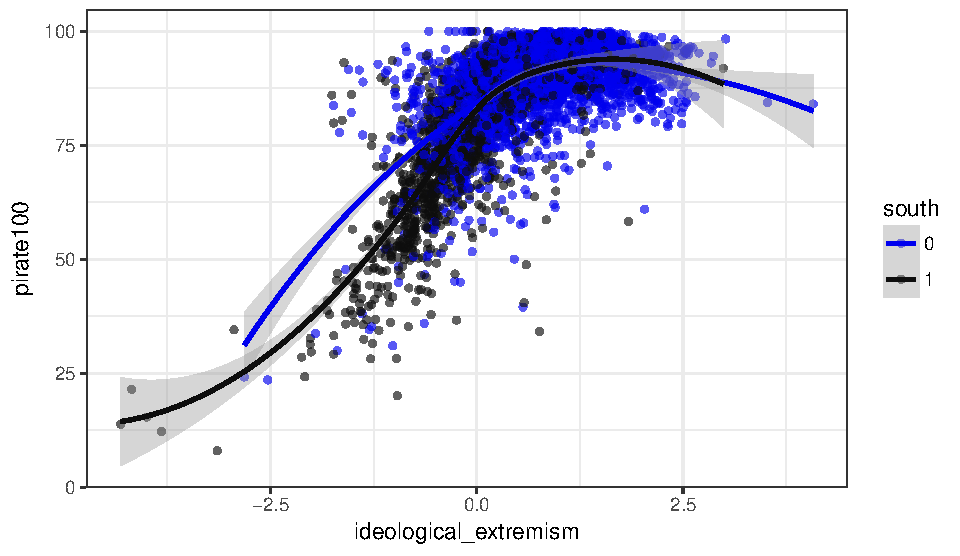
\includegraphics[width = \textwidth]{C:/Users/Ethan/Documents/GitHub/partycalls/plots/house_dem_iv-dv_south_confint.pdf}
\end{figure}

\begin{figure}[H]
	\centering
	\caption{House IV/IV Plot, Republicans, Majority Status}
	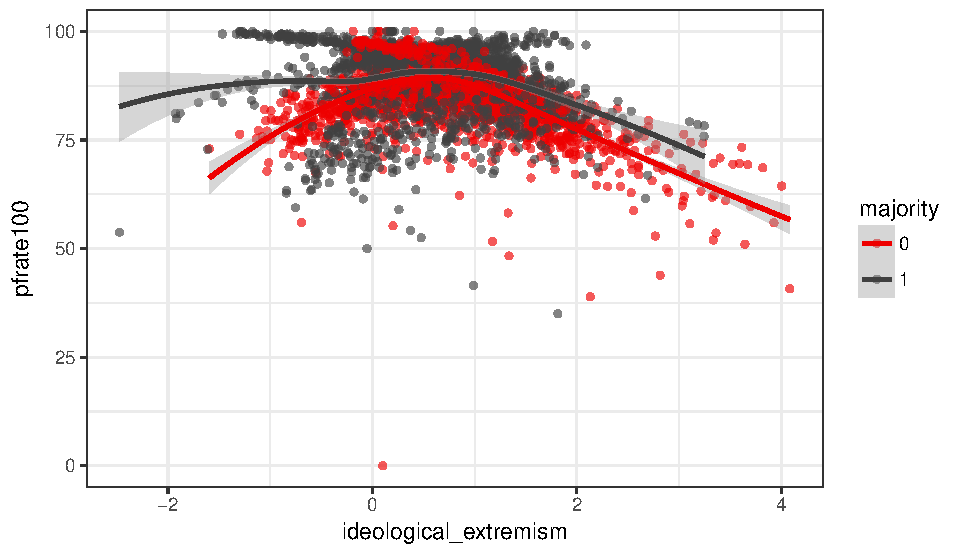
\includegraphics[width = \textwidth]{C:/Users/Ethan/Documents/GitHub/partycalls/plots/house_rep_iv-iv_majority_confint.pdf}
\end{figure}

\begin{figure}[H]
	\centering
	\caption{House DV/IV Plot, Republicans, Majority Status}
	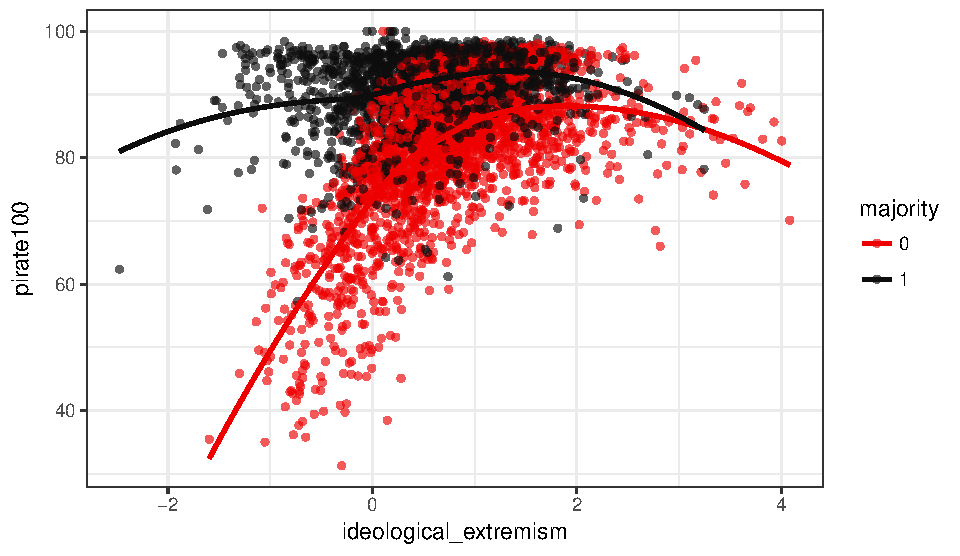
\includegraphics[width = \textwidth]{C:/Users/Ethan/Documents/GitHub/partycalls/plots/house_rep_iv-dv_majority_confint.pdf}
\end{figure}
















\end{document}